\chapter{Lavoro elettrico e Potenziale elettrostatico}

Come vedremo nel seguito, se una carico $q_0$ si muove in presenza di altre cariche, sia fisse che in moto, \emph{la forza su di essa è sempre proporzionale a $q_0$}. Più in generale, quando su una carica $q_0$ agisce una forza $\mathbf{F}$ di qualsiasi natura, non necessariamente elettrostatica, ma ad esempio dovuta a processi chimici o ad azioni meccaniche, o ad altre cause ancora, possiamo definire sempre un campo elettrico $\mathbf{E}$, che si indica con il nome di campo elettromotore \mkeyword{campo elettromotore}, come rapporto tra la forza $\mathbf{F}$ che agisce sulla carica e il calore della carica stessa. In questo modo vale 

\begin{equation*}
    \mathbf{F} = q_0 \mathbf{E}
\end{equation*}

Quindi il lavoro $W_1$ fatto dalla forza $\mathbf{F}$ lungo il percorso $C_1$ ,che porta da un punto $A$ a un punto $B$, risulta essere 

\begin{equation}
    W_1 = \int_{C1} \mathbf{F} \cdot d\mathbf{s} = q_0 \int_{C1} \mathbf{E} \cdot d \mathbf{s} 
    \label{eq: lavoro con campo elettrico}
\end{equation}

In questo modo possiamo andare a definire la tensione elettrica \mkeyword{tensione elettrica} tra i due punti $A$ e $B$ lungo il percorso $C_1$ come

\begin{equation}
    \mathcal{T}_1(A \to B  \ \text{lungo} \ C_1) = \int_{C_1} \mathbf{E} \cdot d \mathbf{s}
\end{equation}

Se si considera un altro percorso $C_2$ si trova in generale un lavoro diverso e quindi un \emph{diverso valore della tensione elettrica}.

\begin{equation*}
    \mathcal{T}_1(A \to B  \ \text{lungo} \ C_1) \neq \mathcal{T}_2(A \to B  \ \text{lungo} \ C_2)
\end{equation*}

Diretta conseguenza di questo è il fatto che in generale il lavoro per un percorso chiuso è diverso da zero. 

\begin{equation}
    W = \oint_C \mathbf{F} \cdot d \mathbf{s} = q_0 \oint_C \mathbf{E} \cdot d \mathbf{s}
\end{equation}

Il lavoro per spostare una carica lungo il percorso chiuso $C$ è dato dal prodotto della carica per la circuitazione del campo elettrico lungo C. \\
L'integrale 

\begin{tcolorbox}[colback=yellow!10!white, colframe=orange!70!black, boxrule=0.8pt]
\begin{equation}
    \mathcal{E} = \oint_C \mathbf{E} \cdot d \mathbf{s}
\end{equation}
\end{tcolorbox}

che esprime il rapporto tra lavoro compiuto sulla carica e la carica stessa per il percorso chiuso $C$ si definisce forza elettromotrice del campo \mkeyword{forza elettromotrice}, f.e.m, relativa al percorso chiuso $C$.

\section{Potenziale elettrostatico}

Se siamo nel caso in cui la forza $\mathbf{F}$ è una forza conservativa, il lavoro compiuto nello spostamento di un punto da $A$ a $B$ è funzione soltanto della posizione di partenza e quella di arrivo e non del cammino seguito. \\
Ne deriva che \emph{il lavoro lungo un qualsiasi percorso chiuso è nullo, ovvero la circuitazione di una forza conservativa è nulla}. \\

Questo è il caso delle forze elettrostatiche, come dimostreremo in seguito. \\
Non dipendendo dal percorso seguito, la tensione elettrica tra il punto $A$ e il punto $B$ può essere espressa come variazione di una funzione \mkeyword{potenziale elettrostatico} delle coordinate, chiamata potenziale elettrostatico :

\begin{tcolorbox}[colback=yellow!10!white, colframe=orange!70!black, boxrule=0.8pt]
\begin{equation}
    V_B - V_A = - \int_A ^B \mathbf{E} \cdot d \mathbf{s}
    \label{eq:definizione_differenza_di_potenziale}
\end{equation}
\end{tcolorbox}

Quindi dalla \ref{eq: lavoro con campo elettrico} risulta 

\begin{equation*}
    W_{AB} = -q_0 (V_B - V_A) = -q_0 \Delta V
\end{equation*}

E per la definizione energia potenziale stessa

\begin{equation*}
    \Delta U = q_0 \Delta V
\end{equation*}

Un'altra conseguenza molto importante è 

\begin{tcolorbox}[colback=yellow!10!white, colframe=orange!70!black, boxrule=0.8pt]
\begin{equation}
    \mathcal{E} = \oint \mathbf{E} \cdot d \mathbf{s}  = 0
\end{equation}
\end{tcolorbox}

\subsection{Calcolo del potenziale elettrostatico}

Andiamo a mostrare che il campo elettrostatico generato da una qualsiasi carica è conservativo. \\

Consideriamo il caso più semplice, quello di una carica puntiforme. 

\begin{equation*}
    dW = q_0 \mathbf{E} \cdot d \mathbf{s} = \frac{q_0\ q}{4\pi \varepsilon_0} \frac{\mathbf{u} \cdot d \mathbf{s}}{r^2} = \frac{q_0\ q}{4\pi \varepsilon_0} \frac{dr}{r^2}
\end{equation*}

Quindi 

\begin{equation}
    W = q_0\int_A ^B \mathbf{E \cdot} d \mathbf{s} = \frac{q_0 \ q}{4 \pi \varepsilon_0} \int_{r_A} ^{r_B} \frac{dr}{r^2} = -q_0 (\frac{q}{4\pi \varepsilon_0r_B}- \frac{q}{4\pi \varepsilon_0 r_A})
    \label{eq:lavoro_carica_puntiforme}
\end{equation}

Abbiamo così verificato che il lavoro non dipende dal percorso seguito. Il risultato era scontato perché la forza in questione è centrale. \\
Dalla \ref{eq:lavoro_carica_puntiforme} si ottiene che 

\begin{equation}
    V_B - V_A = (\frac{q}{4\pi \varepsilon_0r_B}- \frac{q}{4\pi \varepsilon_0 r_A})
    \label{eq:differenza_di_potenziale}
\end{equation}

\newpage

Come l'energia potenziale anche il potenziale è definito a meno una costante additiva e la \ref{eq:differenza_di_potenziale} può essere considerata come la variazione della funzione 

\begin{equation*}
    V(r) = \frac{q}{4 \pi \varepsilon_0r} + C 
\end{equation*}

che rappresenta il potenziale elettrostatico in un punto a distanza $r$ dalla carica $q$.\\

Si può determinare completamente $V(r)$ imponendo la condizione ulteriore:

\begin{equation*}
    r \to +\infty: \quad V(\infty) = 0
\end{equation*}

Come suggerito dal fatto che per cariche molto lontane l'interazione è trascurabile. \\

In conclusione abbiamo che il potenziale elettrostatico generato da una carica puntiforme $q$ in un punto a distanza $r$ vale:

\begin{equation}
    V(r) = - \int_{\infty} ^r \mathbf{E} \cdot d \mathbf{s} = \int_{r} ^{\infty} \mathbf{E} \cdot d \mathbf{s} = \frac{q}{4 \pi \varepsilon_0 r}
\end{equation}

I risultati trovati si estendono senza difficoltà, in base al principio di sovrapposizione, al caso di un campo elettrostatico generato da un numero qualsiasi di cariche puntiformi fisse. 

\begin{figure} [h]
    \centering
    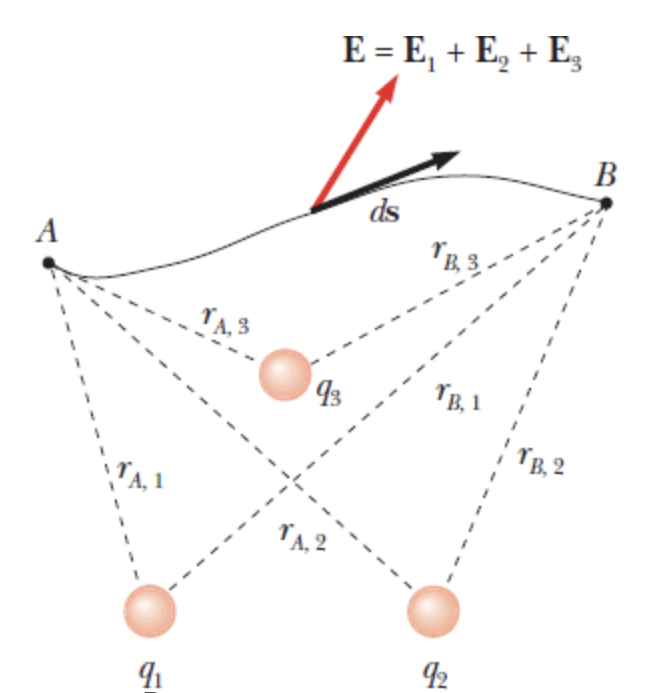
\includegraphics[width=0.45\linewidth]{figure/image4.png}
    \caption{Schema per il calcolo di $\int_A ^B \mathbf{E} \cdot d \mathbf{s}$ per il campo elettrostatico prodotto da un insieme di cariche}  
    \label{fig:calcolo_potenziale_n_cariche}
\end{figure}

\begin{equation*}
    \int_A ^B \mathbf{E} \cdot d \mathbf{s} = \int_A ^B (\sum_i \mathbf{E}_i) \cdot d \mathbf{s} = \sum_i \int_A ^B \mathbf{E}_i \cdot d \mathbf{s} = \sum_i \int_A ^B \frac{q_i}{4 \pi \varepsilon_0 r_i ^2} \mathbf{u}_i \cdot d \mathbf{s}
\end{equation*}

Ciascun integrale porta a un risultato tipo \ref{eq:differenza_di_potenziale} e quindi il campo elettrostatico delle $n$ cariche è conservativo, in particolare risulta che 

\begin{equation}
    V_B - V_A = (\sum_i \frac{q_i}{4 \pi \varepsilon_0 r_{B,i}} - \sum_i \frac{q_i}{4 \pi \varepsilon_0 r_{A,i}})
\end{equation}

E per la convenzione adottata risulta che il potenziale elettrostatico generato dal sistema di cariche nel punto $P(x,y,z)$, distante $r_i$ dalla carica $q_i$, è 

\begin{tcolorbox}[colback=yellow!10!white, colframe=orange!70!black, boxrule=0.8pt]
\begin{equation}
    V(x,y,z) = - \int_{\infty} ^P \mathbf{E} \cdot d \mathbf{s} = \sum_i \frac{q_i}{4\pi \varepsilon_0r_i}
    \label{eq:potenziale_per_più_cariche}
\end{equation}
\end{tcolorbox}

Il potenziale elettrostatico prodotto da un sistema discreto di cariche è uguale alla somma dei potenziali elettrostatici prodotti singolarmente dalle cariche.\\

Nel caso che le cariche siano distribuite in modo continuo basta sostituire nella \ref{eq:potenziale_per_più_cariche} alla sommatoria l'integrale di linea, di superficie o di volume.

\begin{tcolorbox}[colback=yellow!10!white, colframe=orange!70!black, boxrule=0.8pt]
\begin{equation}
    V(x,y,z) = \frac{1}{4\pi \varepsilon_0} \int _{\tau} \frac{\rho (r)}{r} d\tau
    \label{eq:potenziale_senza_condizione}
\end{equation}
\end{tcolorbox}

dove l'integrazione è estesa a \emph{tutte le cariche dell'universo}.

\newpage
